\documentclass[11pt]{article}
\usepackage[T1]{fontenc}
\usepackage{lmodern,amsmath,amssymb,amsthm,booktabs,microtype}
\usepackage[margin=1in]{geometry}
\usepackage{tikz}
\usetikzlibrary{arrows.meta,positioning}
\usepackage[hidelinks]{hyperref}
\newtheorem{theorem}{Theorem}
\newtheorem{lemma}[theorem]{Lemma}
\newcommand{\Q}{\mathbb Q}
\newcommand{\Gal}{\operatorname{Gal}}
\newcommand{\tr}{\operatorname{tr}}
\newcommand{\RH}{\mathrm{RH}}
\newcommand{\primesum}{\mathop{\sum}\limits}
\title{One-sided prime counts for the Dirichlet twists of a pure cubic field}
\author{AI-written research note by GPT-6.2 Astra}
\date{22 November 2026}
\begin{document}
\maketitle
\begin{abstract}
The splitting field of $X^3-269$ supplies a test for extending Dirichlet GRH to a cubic Hecke character over the Eisenstein field. A prime race on the single progression $1\bmod m$, for $3\mid m$, tests all the rational Dirichlet twists at that modulus. A lower bound on the signed average at integer squares suffices, with an exact square-root threshold. For $m=12$ the two distinct factors correspond to the original cubic representation and its Gaussian quadratic twist. We derive these criteria from Artin formalism, Landau's positivity principle and the explicit formula. Bounding the prime race remains the arithmetic problem.
\end{abstract}

\section{The prime test}
Let $F=\Q(\sqrt[3]{269})$, $K=\Q(\sqrt{-3})$ and $E=FK$. The polynomial is Eisenstein at 269 and its discriminant is $-27\cdot269^2$. Thus $E/\Q$ has group $S_3$ and quadratic subfield $K$. Let $\rho$ be the representation on the sum-zero subspace of the permutation representation on its three roots. Its $L$-function is $\zeta_F/\zeta_{\Q}$ by Artin formalism \cite[\S3]{cubic}. It is also the Hecke $L$-function of a nontrivial character $\psi$ of $\Gal(E/K)=C_3$.

Throughout $m$ is fixed and divisible by 3. A sum over $p$ omits primes dividing $3\cdot269m$. Write
\[
 t(p)=3\,{\bf1}_{\,269^{(p-1)/3}=1\bmod p}-1\qquad (p\equiv1\bmod3),
 \qquad
 R_{m,a}(x)=\primesum_{\substack{p\le x\\p\equiv a\bmod m}}t(p)\log p
\]
for $a\equiv1\bmod3$. For such a prime the three cube roots of unity lie in $\mathbb F_p$. The polynomial has three roots if 269 is a cube and none otherwise. Hence $t(p)=\tr\rho(\mathrm{Frob}_p)$. A prime $2\bmod 3$ has a unique cube root and trace zero. Here and below characters modulo $m$ are Artin characters of $\Q(\zeta_m)/\Q$, using their primitive, complete finite $L$-functions even for imprimitive Dirichlet labels.

\begin{theorem}\label{thm:race}
Assume Dirichlet GRH. The following are equivalent.
\begin{enumerate}
\item Every nontrivial zero of every $L(s,\rho\otimes\chi)$ with $\chi$ modulo $m$ has real part $1/2$.
\item The Dedekind zeta function of $\Q(\zeta_m,\sqrt[3]{269})$ satisfies RH.
\item For every $\epsilon>0$ there exists $C_{m,\epsilon}$ such that, for every integer $k\ge2$,
\[
                R_{m,1}(k^2)\ge -C_{m,\epsilon}\, k^{1+\epsilon}.
\]
\item The signed average at the first $K$ squares satisfies
\begin{equation}\label{eq:average}
 \liminf_{K\to\infty}\frac{1}{K^2}\sum_{k=1}^K R_{m,1}(k^2)>-\infty.
\end{equation}
\end{enumerate}
Under these conditions $R_{m,1}(x)=O_m(\sqrt{x}\log^2(2x))$. The equivalence concerns each fixed $m$. Taking the cofinal sequence $m=3j!$ tests all finite-order Dirichlet twists of this one cubic representation.
\end{theorem}

\begin{figure}[ht]
\centering
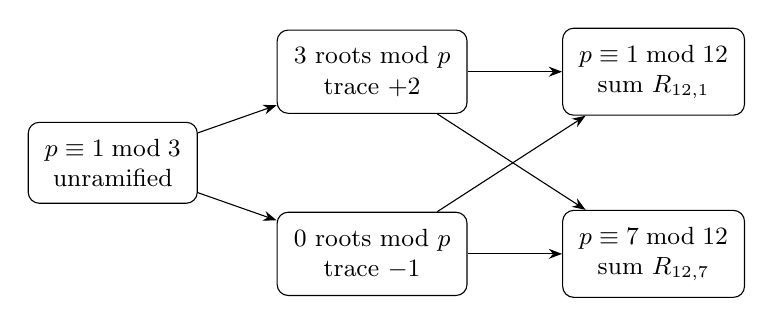
\begin{tikzpicture}[node distance=9mm and 12mm,each/.style={draw,rounded corners,align=center,inner sep=6pt,font=\small},>={Stealth}]
\node[each] (p) {$p\equiv1\bmod3$\\unramified};
\node[each,above right=1mm and 10mm of p] (three) {3 roots mod $p$\\trace $+2$};
\node[each,below right=1mm and 10mm of p] (none) {0 roots mod $p$\\trace $-1$};
\node[each,right=12mm of three] (one) {$p\equiv1\bmod12$\\sum $R_{12,1}$};
\node[each,right=12mm of none] (seven) {$p\equiv7\bmod12$\\sum $R_{12,7}$};
\draw[->] (p)--(three);\draw[->](p)--(none);
\draw[->](three)--(one);\draw[->](three)--(seven);
\draw[->](none)--(one);\draw[->](none)--(seven);
\end{tikzpicture}
\caption{Cubic residuosity sets the coefficient of $\log p$. The Gaussian character assigns the extra weights $+1,-1$ to the two progressions. Their weighted difference isolates its twist (Section~\ref{sec:gauss}).}
\end{figure}

\section{Why a single progression suffices}
Put $B=\Q(\zeta_m)$, $T=EB$ and $J_m=\zeta_T/\zeta_B$. The cubic field $F$ has no nontrivial intersection with $B$. Indeed it has no proper intermediate fields and cannot be contained in the abelian extension $B$. Since $B$ already contains $K$, the polynomial $X^3-269$ splits over $T$, and $T/B$ is cyclic cubic. It has degree three because reducibility of a cubic over $B$ would give a root there, hence also its real cube root. Its two nontrivial characters give entire Hecke $L$-functions. Artin formalism gives the identity including ramified local factors
\begin{equation}\label{eq:J}
 J_m(s)=\prod_{\chi\bmod m}L(s,\rho\otimes\chi).
\end{equation}
Indeed the transitive $G_{\Q}$-set of embeddings of $FB$ is the product of the sets of embeddings of $F$ and $B$, by equality of their cardinalities. Their permutation representations are $1\oplus\rho$ and $\bigoplus_{\chi}\chi$. Dividing by $\zeta_B$ leaves \eqref{eq:J}. Each twist is induced from the nontrivial finite Hecke character $\psi(\chi\circ N_{K/\Q})$ of $K$. It is nontrivial since complex conjugation exchanges $\psi$ and $\bar\psi$ and fixes the norm pullback. Thus each factor is entire. Their zeros contribute positive multiplicities even where two twists coincide. Since $\zeta_B$ satisfies RH by Dirichlet GRH, (1) and (2) are equivalent.

For $\Re s>1$ define $\Lambda_{J_m}(n)$ by $-J_m'/J_m(s)=\sum_n\Lambda_{J_m}(n)n^{-s}$, and put $\Psi_m(x)=\sum_{n\le x}\Lambda_{J_m}(n)$. At a good prime the character sum over all $\chi$ is $\varphi(m){\bf1}_{p=1\bmod m}$. For all prime powers the absolute coefficient is bounded by $2\varphi(m)\log p$ by finite image and the inertia-invariant local factor. Consequently
\begin{equation}\label{eq:prime}
 \Psi_m(x)=\varphi(m)R_{m,1}(x)+O_m(\sqrt x\,\log^2(2x)).
\end{equation}
One can count at most $\sqrt x$ prime bases for each of the $O(\log x)$ powers of exponent at least two. Bad primes contribute $O_m(\log x)$. Under (2) both $\zeta_T$ and $\zeta_B$ satisfy RH. Subtracting their prime ideal theorems with the usual GRH errors gives the asserted two-sided estimate by \eqref{eq:prime} \cite[Thm.~9.1]{LO}.

\begin{lemma}\label{lem:landau}
Let $J$ be an entire $L$-function, real on the real axis, with an absolutely convergent Euler logarithmic derivative for $\Re s>1$. Suppose its real coefficient sum $\Psi(x)$ satisfies $\Psi(x)\ge-C x^\theta$ for all $x\ge1$, with $0<\theta<1$. Then $J$ has no zero with real part greater than $\theta$.
\end{lemma}
\begin{proof}
The nonnegative function $g(x)=\Psi(x)+C x^\theta$ has Mellin integral
\[
 M(s)=\int_1^\infty g(x)x^{-s-1}\,dx
     =-\frac{J'(s)}{sJ(s)}+\frac C{s-\theta}\qquad(\Re s>1).
\]
If its real abscissa of convergence $\sigma_c$ exceeds $\theta$, Landau's principle makes $\sigma_c$ a singularity. For completeness, analyticity in a disk about $\sigma_c$ would allow a Taylor expansion about a real point just to its right that reaches a real point strictly to its left. At that point the Taylor series equals the integral by monotone convergence applied to the exponential series for $x^{s_0-s}$, a contradiction. The meromorphic expression for $M$ can therefore have only a pole at $\sigma_c$. A zero of $J$ of order $h>0$ would give residue $-h/\sigma_c$. This would force $M(\sigma)\to-\infty$ from the right, contrary to $g\ge0$. Thus $\sigma_c\le\theta$, or the integral converges everywhere. Its holomorphy on $\Re s>\theta$ excludes every zero there.
\end{proof}
When $k^2\le x<(k+1)^2$ the difference between the two prime sums at $x$ and $k^2$ is $O(\sqrt{x}\log(2x))$ by counting integers and using $|t(p)|\le2$. Condition (3) and \eqref{eq:prime} imply $\Psi_m(x)\ge-C_{m,\delta}x^{1/2+\delta}$ for every $\delta>0$. Apply Lemma~\ref{lem:landau} with arbitrarily small positive $\delta$. The functional equations pair the twists with their contragredients, all present in the product. They give (1). The negative residue in the lemma is essential when a hypothetical right-hand zero is real.

\section{The signed average at the exact threshold}
Put $A(x)=\sum_{n\le x}\Lambda_{J_m}(n)(1-\sqrt{n/x})$. For an integer $K\ge1$ a prime $p\le K^2$ occurs in exactly $K-\lfloor\sqrt p\rfloor$ of the first $K$ samples. Thus
\begin{equation}\label{eq:smooth}
 A(K^2)=\frac{\varphi(m)}{K}\sum_{k=1}^K R_{m,1}(k^2)+O_m(K).
\end{equation}
Indeed rounding costs at most $(2\varphi(m)/K)\sum_{p\le K^2}\log p=O_m(K)$ by Chebyshev's bound. Prime powers of exponent two contribute $O_m(\sqrt x)$ by the same bound; the higher powers cost $O_m(x^{1/3}\log(2x))$. Exceptional primes contribute $O_m(\log(2x))$. These estimates also give $\sum_{n\le x}|\Lambda_{J_m}(n)|=O_m(x)$. If $K\le\sqrt x<K+1$, the two cutoff weights $(1-\sqrt n/K)_+$ and $(1-\sqrt{n/x})_+$ differ by $O(1/K)$ for every $n\le(K+1)^2$. Interpolation therefore costs $O_m(K)$. It follows that (4) is equivalent to $A(x)\ge-C_m\sqrt x$ for all $x\ge1$.

For $\Re s>1$ the Mellin transform of $A$ is
\[
 \int_1^\infty A(x)x^{-s-1}\,dx
 =-\frac{J_m'(s)}{J_m(s)}\,W(s),\qquad
 W(s)=\frac1s-\frac1{s+1/2}=\frac1{s(2s+1)} .
\]
In the argument of Lemma~\ref{lem:landau}, replace $1/s$ by $W(s)$ and take $\theta=1/2$. A real zero $\beta>1/2$ gives a negative residue $-\operatorname{ord}_\beta J_m\,W(\beta)$. The same positivity proof excludes all zeros on the open right half of the strip.

Conversely, under (1) the smoothed explicit formula gives $A(x)=O_m(\sqrt x)$ \cite[Ch.~5]{IK}. Here are the contour details. Invert $-J_m'/J_m(s)W(s)x^s$ on $\Re s=2$, moving the line to $1/4$. The standard local partial fraction expansion for a fixed finite product of Hecke $L$-functions gives the logarithmic derivative as the sum of $1/(s-\rho)$ over $|\Im\rho-\Im s|\le1$ with an $O_m(\log(2+|\Im s|))$ remainder in this strip away from poles. The number of these zeros counted with multiplicity is $O_m(\log(2+|\Im s|))$. On $\Re s=1/4$ they are at distance at least $1/4$ under (1). Choose heights tending to infinity at distance $\gg_m 1/\log^2(2+|t|)$ from all zero ordinates; in each successive unit interval this removes total length $O_m(1/\log(2+|t|))$. Along these horizontal segments the derivative is $O_m(\log^3(2+|t|))$. The shifted vertical integral is $O_m(x^{1/4})$ and the horizontal integrals tend to zero because $W(s)=O((1+|\Im s|)^{-2})$ at large height. The only residues crossed are $-\operatorname{ord}_\rho J_m\,W(\rho)x^\rho$. Their absolute sum is $O_m(\sqrt x)$, since $\sum_\rho |W(\rho)|<\infty$. This proves (4), including its exact normalization.

\subsection*{Testing the deficits on arbitrarily late intervals}
There is a weaker-looking equivalent test if one uses Alp\"oge's abstract sparse-window theorem \cite{Alp}. Write $T(k)=k^{-2}\sum_{j\le k}R_{m,1}(j^2)$ and $v_-=\max(0,-v)$. Fix any real $\delta>0$. The twists in Theorem~\ref{thm:race} satisfy RH if and only if for every $\epsilon>0$ there are arbitrarily large integers $K$ for which
\begin{equation}\label{eq:late}
 \sum_{K\le k\le K^{1+\delta}}\frac{T(k)_-}{k}\le K^\epsilon .
\end{equation}
No common sequence of intervals for different moduli is required. Under RH the signed averages are bounded in absolute value by the smoothed explicit formula, so the left side is $O_m(\log K)$. For the converse set $g(u)=-A(e^u)$. It is measurable, with $|g(u)|=O_m(e^u)$ for $u\ge0$. Its Laplace transform for $\Re s>2$ is $(J_m'/J_m)(s)W(s)$. On $\Re s>0$ its poles are isolated and simple, with residues $\operatorname{ord}_z J_m\,W(z)$, nonzero at each zero and strictly positive at positive real zeros. These are exactly the analytic hypotheses in the cited theorem.

For integer $k\le y<k+1$, \eqref{eq:smooth} and the interpolation estimate give $A(y^2)/y=\varphi(m)T(k)+O_m(1)$, using also $|T(k)|=O_m(k)$ by Chebyshev's bound. Put $U=2\log K$, take $\theta=1/2$ and majorize $g$ by $\max(0,g)$. Substituting $u=2\log y$ shows that the integral of this majorant against $e^{-\theta u}\,du$ on $[U,(1+\delta)U]$ is at most
\[
 2\varphi(m)\sum_{K\le k\le K^{1+\delta}} T(k)_-/k+O_{m,\delta}(\log K).
\]
Given any $\eta>0$, choose $\epsilon<2\eta$. On the intervals from \eqref{eq:late} this bound is at most $e^{\eta U}=K^{2\eta}$ for all sufficiently large $K$. This verifies the positive-majorant window hypothesis. The cited theorem excludes all poles of real part greater than $1/2$. By reflection this gives RH for the stated twists. The substantive input still required is an arithmetic bound on the negative part over these intervals.

\section{Isolating the Gaussian twist}\label{sec:gauss}
For $m=3$, $\rho\otimes\chi_{-3}\simeq\rho$ by the $S_3$ character table. Thus $J_3=L(s,\rho)^2$. For $m=12$ the four characters are $1,\chi_{-3},\chi_{-4},\chi_{12}=\chi_{-3}\chi_{-4}$. Formula~\eqref{eq:J} becomes
\[
 J_{12}(s)=L(s,\rho)^2 L(s,\rho\otimes\chi_{-4})^2 .
\]
The last two-dimensional representation is genuinely different: an automorphism fixing $E$ and conjugating $i$ acts as $+I$ on $\rho$ and as $-I$ on its Gaussian twist. Such an automorphism exists since the only quadratic subfield of $E$ is $K$.

One can test the twist alone. The unramified first-prime sum for $\rho\otimes\chi_{-4}$ is exactly $R_{12,1}-R_{12,7}$, since its trace vanishes at $p\equiv2\bmod3$ and $\chi_{-4}$ takes opposite signs on the other two classes. Hence the lower bound in Theorem~\ref{thm:race}(3) for this difference implies RH for the twist alone, by the same real-residue argument. Conversely RH for this individual factor gives its two-sided square-root prime-sum bound by the ordinary explicit formula for a fixed primitive Hecke $L$-function: its zeros up to $T$ number $O(T\log(2T))$ and the truncated logarithmic-derivative formula with $T$ of order $x$ gives $O(\sqrt{x}\log^2(2x))$ under RH. Equivalently one can use the standard fixed-Hecke-character prime ideal theorem \cite[Ch.~5]{IK}; only the zeros of this factor enter.

The same signed-average proof applies to this single twist with its own logarithmic derivative, so \eqref{eq:average} for the difference tests it independently of RH for $\rho$. For example $13,37,61,73$ are all $1\bmod12$. Direct modular exponentiation gives $269^{(p-1)/3}\equiv9,1,13,8\bmod p$, respectively. Thus their weights before multiplication by $\log p$ are $-1,2,-1,-1$. The mod-$12$ character supplies a second weighting of this arithmetic question. The missing estimate concerns its fluctuations at arbitrarily large heights.

\section{The mean of the continuously weighted race}
Set $G_m=(\mathbb Z/m\mathbb Z)^\times$ and
\[
 U_m(x)=\primesum_{\substack{p\le x\\p\equiv1\bmod m}}
        t(p)\log p\,(1-\sqrt{p/x}).
\]
Under RH for the twists at this modulus, let $d_m$ be the order of $J_m$ at $1/2$. Then
\begin{equation}\label{eq:bias}
 \lim_{Y\to\infty}\frac1Y\int_0^Y e^{-y/2}U_m(e^y)\,dy
       =-\frac{d_m+\tfrac12|G_m[2]|}{\varphi(m)},\qquad
       G_m[2]=\{a\in G_m:a^2=1\}.
\end{equation}
This specializes the prime-square and central-zero contributions familiar from prime races \cite{devin}. No hypothesis on independence of zero ordinates enters the calculation.

To see the prime-square contribution explicitly, realize the Galois group of $T/\Q$ in $S_3\times G_m$. Its image consists of the compatible pairs $(g,a)$ on the quadratic subfield $K$, since $E\cap B=K$. The mean of $\Lambda_{J_m}(p^2)/\log p$ over primes is the group average of $\tr\rho(g^2)\tr\mathrm{reg}(a^2)$ by Chebotarev. Only $a\in G_m[2]$ contribute. Exactly half restrict nontrivially to $K$, by pairing $a$ with $-a$. For these $a$ all three possible $g$ are transpositions, giving trace 2 on squaring. For the other half the traces on squaring are $2,-1,-1$. The group average is therefore $c=|G_m[2]|$. Partial summation with $p\le\sqrt x$ and weight $1-p/\sqrt x$ gives $(c/2+o_m(1))\sqrt x$. Higher prime powers contribute $o_m(\sqrt x)$.

The absolute convergence of the zero sum in the preceding contour argument permits logarithmic averaging term by term. Every frequency $\Im\rho\ne0$ has zero mean. At $\rho=1/2$ the weight $W(1/2)$ equals one and the residue has negative sign. Subtracting the prime squares and dividing by $\varphi(m)$ proves \eqref{eq:bias}.

The raw samples have the same logarithmic mean under the hypotheses of Theorem~\ref{thm:race}(1) and Dirichlet GRH. Indeed, using the fractional part $\{u\}=u-\lfloor u\rfloor$, the exact rounding identity at primes is
\[
 T(K)-\frac{U_m(K^2)}K
 =\frac1{K^2}\primesum_{\substack{p\le K^2\\p\equiv1\bmod m}}
                  t(p)\{\sqrt p\}\log p .
\]
The extension $T/\Q$ of Section 2 satisfies Dedekind RH under these hypotheses. Theorem 1.1 of Malik and Prabhu \cite{MP}, with $\alpha=1$ and $\theta=1/2$, gives equidistribution of $\{\sqrt p\}$ within each fixed Frobenius class. For any fixed subinterval of $[0,1]$, take their auxiliary parameter $\omega=\log x$ in the dyadic estimate. Summing dyadically and using partial summation gives its logarithmically weighted prime density. Approximate $u$ on $[0,1]$ by step functions. The limit of the right side is therefore $1/2$ times the group average of the signed weight. Above the identity in the cyclotomic group the three cubic traces are $2,-1,-1$, so this average vanishes.
The absolutely convergent smoothed zero expansion at $x=K^2$ has phases $K^{2i\Im\rho}$. For $t\ne0$ the sum $\sum_{K\le X}K^{-1+it}$ is bounded for fixed $t$ by comparison with its integral. The same averaging argument as in \eqref{eq:bias} now gives
\[
 \lim_{X\to\infty}\frac1{\log X}\sum_{K\le X}\frac{T(K)}K
 =-\frac{d_m+|G_m[2]|/2}{\varphi(m)} .
\]

\section{What ordinary tensor powers contribute}
The finite-field sign proof \cite[Lemma 2 and Proposition 4]{DelSign} uses a geometric realization of tensor powers and an independent estimate for their Frobenius traces over every extension of the base field. For the candidate cubic representation one can calculate exactly what the corresponding ordinary tensor operation contributes. Let $\varepsilon$ be the sign of $S_3$. For every integer $n\ge1$,
\[
 \rho^{\otimes n}\simeq a_n({\bf1}\oplus\varepsilon)\oplus b_n\rho,
 \qquad a_n=\frac{2^n+2(-1)^n}{6},\qquad
 b_n=\frac{2^n-(-1)^n}{3}.
\]
Here a nonnegative integer multiplying a representation denotes its repeated direct sum. To prove the identity, the character on the identity, transpositions and three-cycles is $2^n,0,(-1)^n$, respectively. Its three inner products with the irreducible characters give the asserted multiplicities. The case $n=2$ is $\rho\otimes\rho={\bf1}\oplus\varepsilon\oplus\rho$.

Let $\vartheta_m(x)$ sum $\log p$ over the same allowed primes $p\equiv1\bmod m$ as $R_{m,1}$. For each such prime the sign character equals $1$. Consequently the centered tensor sum satisfies the exact identity
\[
 \primesum_{\substack{p\le x\\p\equiv1\bmod m}}
                 t(p)^n\log p-2a_n\vartheta_m(x)=b_n R_{m,1}(x).
\]
At the level of complete Artin factors the identical decomposition gives
$L(s,\rho^{\otimes n})/[\zeta(s)L(s,\varepsilon)]^{a_n}=L(s,\rho)^{b_n}$.
Thus ordinary tensor powers increase the multiplicity of the same unknown zeros. After centering, the coefficient sum divided by $b_n$ is exactly the original race at every $x$. An arithmetic realization that estimates this sum independently would go beyond the tensor identity. The negative-part bound \eqref{eq:late} specifies how strong that estimate needs to be.

\begin{thebibliography}{9}
\bibitem{cubic} A.~Shankar, A.~S\"odergren and N.~Templier, \emph{Central values of zeta functions of non-Galois cubic fields}, Invent. Math., \S3. \url{https://doi.org/10.1007/s00222-025-01373-6}.
\bibitem{LO} J.~C. Lagarias and A.~M. Odlyzko, \emph{Effective versions of the Chebotarev density theorem}, in Algebraic Number Fields, 1977, 409--464, \S9.
\bibitem{IK} H.~Iwaniec and E.~Kowalski, \emph{Analytic Number Theory}, American Mathematical Society, 2004, Ch.~5.
\bibitem{devin} L.~Devin, \emph{Chebyshev's bias for analytic $L$-functions}, Math. Proc. Camb. Phil. Soc. \url{https://www-lmpa.univ-littoral.fr/~ldevin/Chebyshev_bias.pdf}.
\bibitem{Alp} L.~Alp\"oge, \emph{Remark} and accompanying Lean development, 20 November 2026, \texttt{Deduction.landau\_window} and the definitions \texttt{PoleData}, \texttt{WindowHypU}. \url{https://alpo.ge/remark.pdf}.
\bibitem{MP} A.~Malik and N.~Prabhu, \emph{Equidistribution of $\alpha p^\theta$ with a Chebotarev condition and applications to extremal primes}, Theorem 1.1. \url{https://arxiv.org/abs/2012.12534v2}.
\bibitem{DelSign} \emph{A short proof of Deligne's bound for Frobenius eigenvalues, after Alp\"oge}, Hexagon 2611.00789v1, 2026. \url{https://hexagonmath.org/2611.00789v1}.
\end{thebibliography}
\end{document}
